%Simulation Results and Discussion


The shortest tour length is calculated in different \textit{rounds} for a 30 and 51 cities problem (called \emph{oliver30} and \emph{eil51} respectively) and averaged over 10 \textit{trials}. Whereas one \textit{round} means that every agent \textit{once} walked through all cities in the network and for the next \textit{round} the agents start with the update pheromone on their tours and one \textit{trial} means that all agents have completed a certain amount of \textit{rounds} and found a shortest path. For the next \textit{trial} everything is set to the initial conditions and at the end the average of the shortest paths found in the different trials is taken. The error bars in the following plots always refer to the standard deviation from those repeated measurements.\\
The distances between the cities are determined using the given coordinates on a two dimensional euclidean plane. The distance $d_\text{i,j}$ between city $i$ and $j$ is then calculated by (\textit{calc\_Lnn.m})
\begin{equation}
d = \sqrt{(x_i-x_j)^2+(y_i-y_j)^2}.
\label{eq:dist}
\end{equation}
For \emph{oliver30} the distances are rounded to the next integer values, whereas in \emph{eil51} double distances are used. This leads to slightly different numbers for the shortest tour length.\\
\subsection{Length of shortest tour}
The trajectory vector of the shortest tour is defined as the sequence of city numbers which yields the optimal tour length.\\
For the city environment \emph{oliver30} the solution found in [3] is given by $[1,~3,~  4,~  5,~  6,~  7,\\~  8,~  9,~  10,~  11,~  12,~  13,~  14,~  15,~  16,~  17,~  18,~  19,~  20,~  21,~  22,~  23,~  25,~  24,~  26,~  27,~  28,~  29,$\\$  30,~  2]$. Using equation (\ref{eq:dist}) the total tour length is calculated to $shortest~path_\text{solution} = 420$. Comparing it to the sequence obtained from own simulations one observes a somewhat different sequence: $[1, ~2,~3,~  4,~  5,~  6,~  7,~  8,~  9,~  10,~  11,~  12,~  13,~  14,~  15,~  16,~  17,\\  18,~  19,~  20,~  21,~  22,~  23,~  25,~  24,~  26,~  27,~  28,~  29,~  30]$ where the agents do not move from city 30 to 2 but to 1. However, the length of this shortest path also results in $shortest~ path_\text{simulation}=420$. Obviously, there exist two solutions to this symmetric TSP using rounded distances.\\
\begin{figure}[H]
\begin{center}
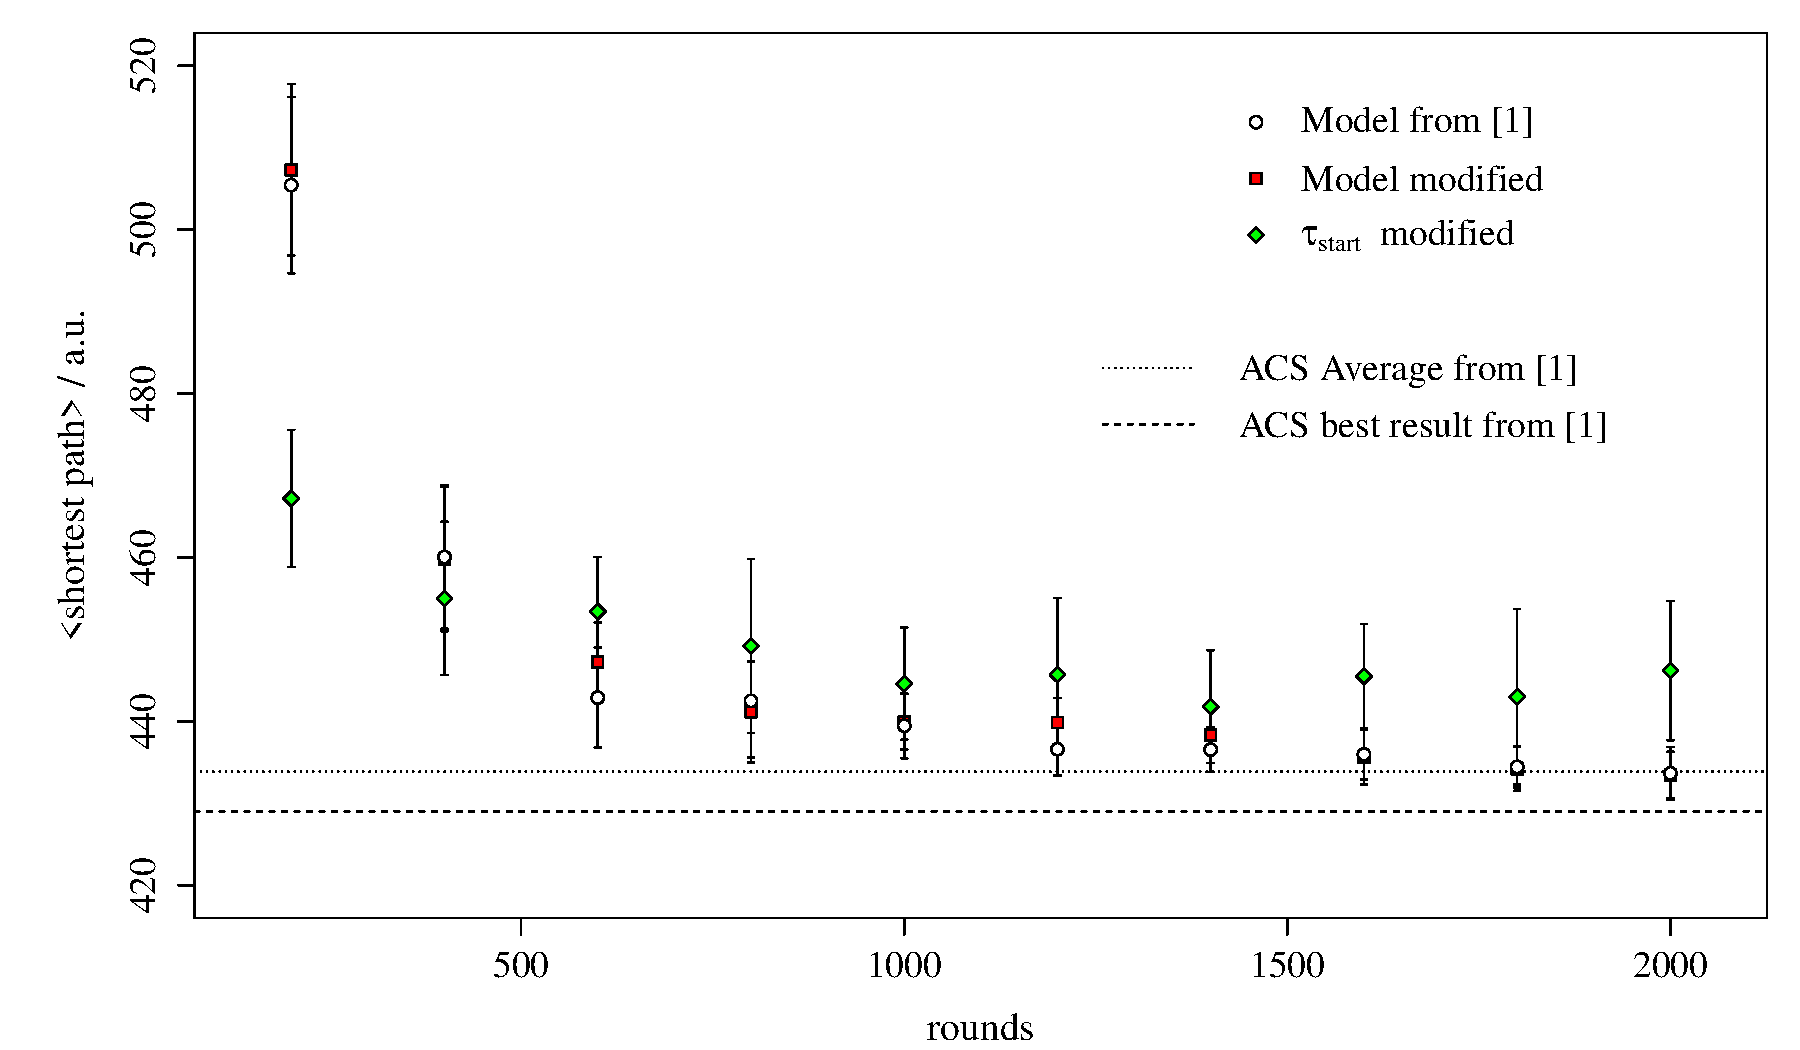
\includegraphics[width= 1\linewidth]{rounds_vs_shortestpath_eil}
\caption{Shortest tour length averaged over 10 trials for different numbers of rounds and 10 agents with the corresponding standard deviation as error bars for problem \textit{eil51}. Thereby two slightly different implementations of the model from literature [1] are done (white circle dots and red squares, see text). The green diamonds correspond to a model where the update formula $\tau(r,s)$ is changed (equation 5). The values approximate the optimal solution for $\approx$ 1200 rounds. The two different lines represent the best shortest tour and the average value measured according to [1]. The parameters are chosen as follows $\alpha=0.1$, $\beta=2$, $q_0=0.9$, $\tau_\text{start}=0.1$.}
\label{fig:roundspeil}
\end{center}
\end{figure}
\noindent In Figure \ref{fig:roundspeil} and \ref{fig:roundspoli} the dependency of the shortest path length on the number of completed rounds is shown. As expected the average length decreases asymptotically towards the value of the optimal path. For \emph{oliver30} $<$shortest~path$>$ is in fact equal to the best result found using 400 rounds, whereas in \emph{eil51} a lot more rounds would have been needed to achieve this. Anyhow, the best result obtained for \emph{eil51} in a single run is $shortest~path_{\text{simulation}}=429.48$. Comparing the ACS average path length and best yielded result to values from literature ([1] and [3]) one concludes that the implementation of the model was a full success (table \ref{tab:val}). For both problems the optimal tour length is found and the average value in \emph{eil51} is similar to the one from literature\footnote{Unfortunately there are no confidential intervals given in [1].}.

\begin{table}[h!]
%\setlength{\tabcolsep}{5pt}
\renewcommand{\arraystretch}{1.2}
\center
\begin{tabular}{|c|c|c|c|c|}
	\hline
		&ACS average				&		ACS best result				& 	ACS average		&	ACS best result \\
		&[1] and [3]	&		[1] and [3]		&	simulation	&	simulation \\\hline	
	
		\emph{eil51}	&  433.87	&	429 	& $433.7 \pm 3.2$ & 429.48 	\\\hline
		\emph{oli30}	&  (N/A)	  	&	420		& $420.5 \pm 0.5$ & 420		\\\hline
		

		
\end{tabular}
\caption{Simulation results of two city environments compared to values from literature ([1] and [3]). Own simulations: \emph{eil51} the agents completed 2000 rounds, for \emph{oli30} 400. Literature: \emph{eil51} the agents completed 500 rounds, for \emph{oli30} there is no average shortest path length determined.}
\label{tab:val}
\end{table}
\noindent In Figure \ref{fig:roundspeil} three models have been implemented and tested. The first (white circle dots) correspond exactly to the one described in [1] where all agents are moving at the same time step. The red squares represent the result obtained by a slightly modified implementation. The same mathematics has been used but the agents are exploring a new trail one by one (see chapter \ref{sec:model}). As can be seen, this change has little effect on the value of the shortest tour length and its error.\\ Adapting the pheromone update equation (\ref{eq:globalupdate}) on page \pageref{eq:globalupdate} by adding a constant of 0.1 (as described in chapter \ref{sec:model}) does not result in better values for the shortest path. On the contrary it seems this model will not easily find the shortest path at a reasonable number of rounds. One concludes that this type of rewarding the shortest path is quite likely to end in a local minimum where it cannot get out due to the local shortest path being rewarded more and more after every round.\\

\begin{figure}[H]
\begin{center}
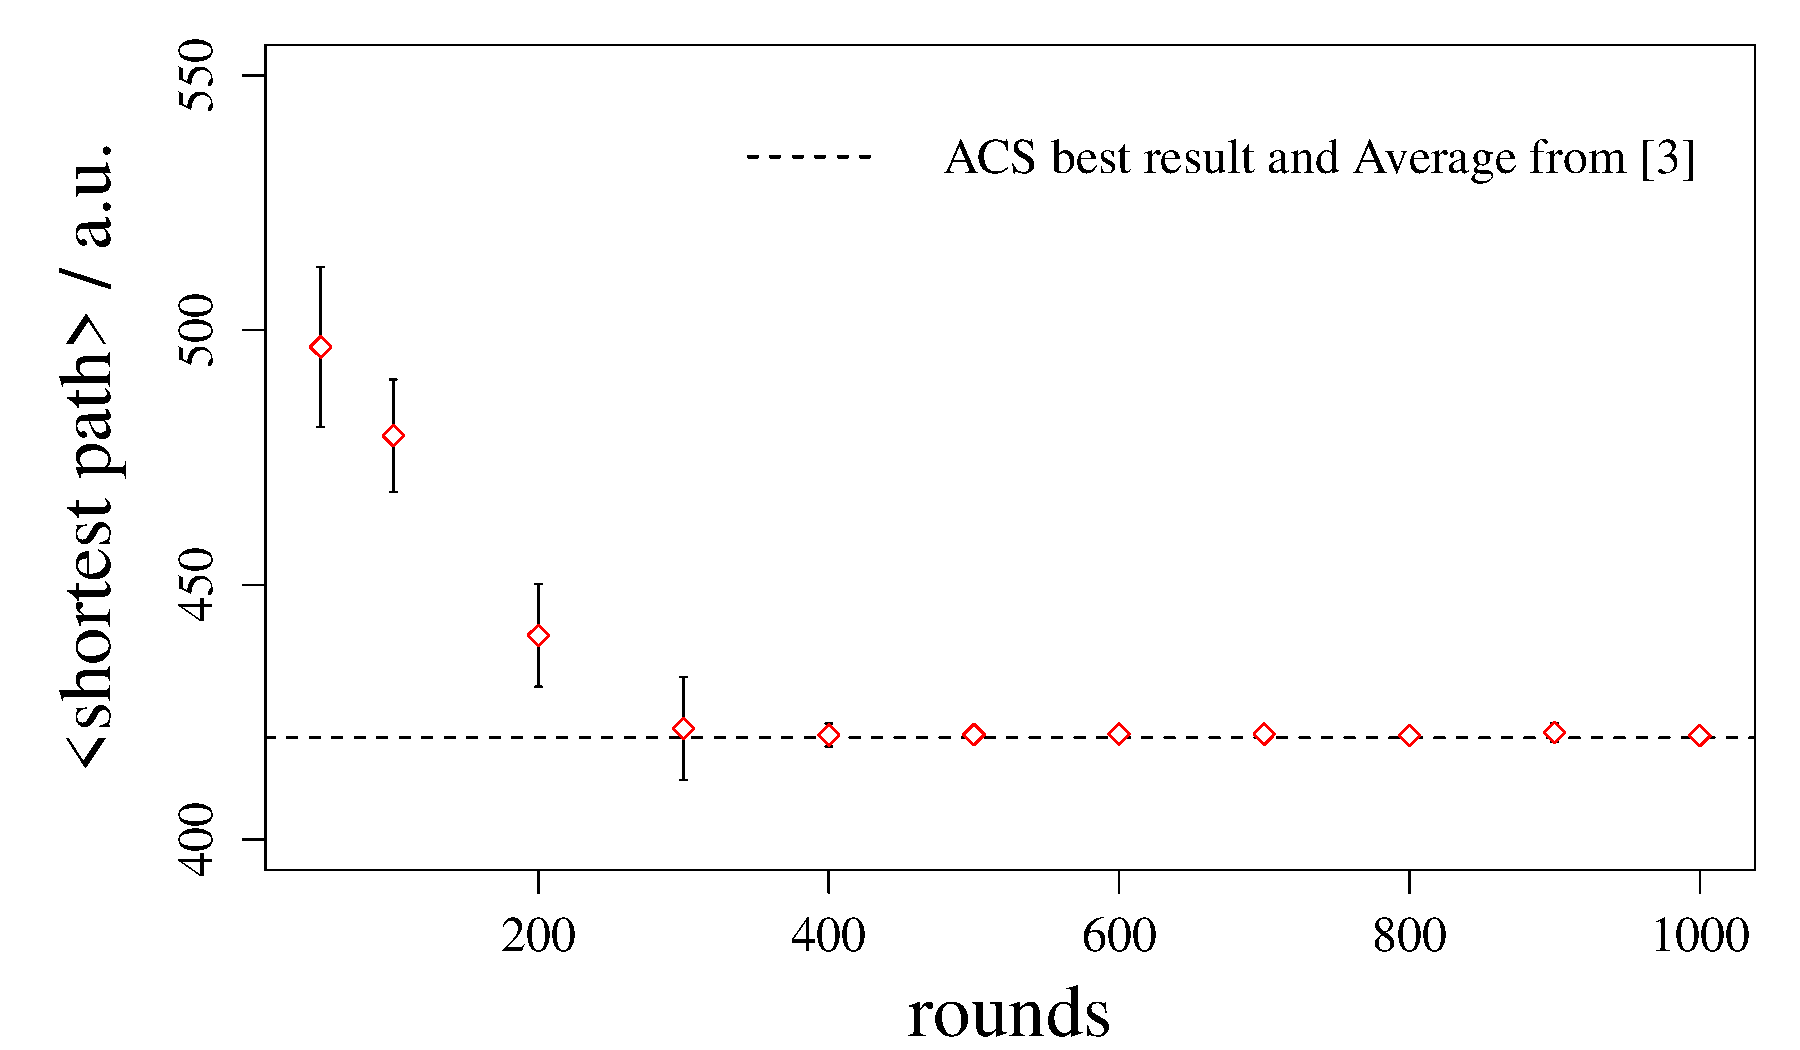
\includegraphics[width=1\linewidth]{rounds_vs_shortestpath_oli}
\caption{Shortest tour length averaged over 10 trials for different numbers of rounds and 10 agents with the corresponding standard deviation as error bars for problem \textit{olvier30}. The value approximates the optimal solution at $\approx$ 400 rounds. For this simulation the model and its implementation are done in the same way as in [1].}
\label{fig:roundspoli}
\end{center}
\end{figure}
\begin{figure}[H]
\begin{center}
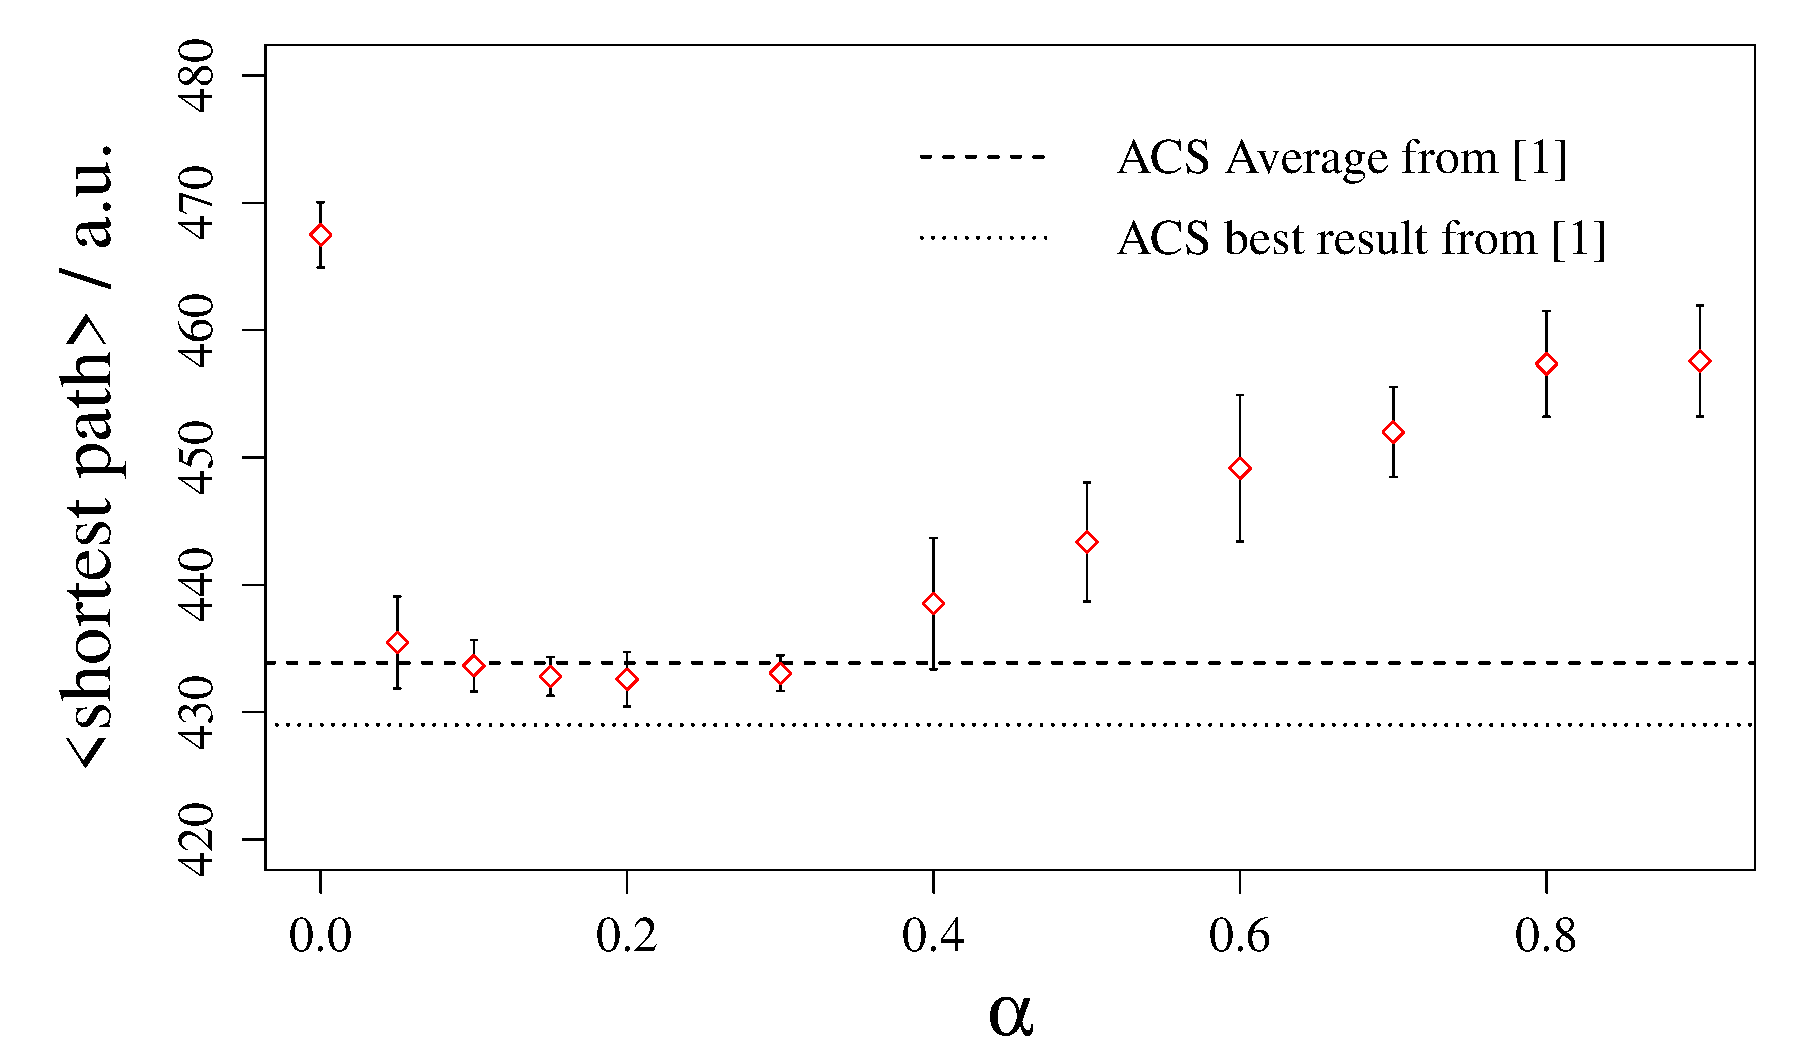
\includegraphics[width=1\linewidth]{alpha_vs_shortestpath}
\caption{The update rate parameter $\alpha$ changes the averaged shortest tour length. The simulation is done for a 51-city problem using ten agents which all completed 2000 rounds. Other parameters are set to $\beta=2$, $q_0=0.9$ and $\tau_{start}=0.1$. The values are averaged over ten trials. By setting $\alpha=0.1$ the length of the averaged shortest path is comparable to the value found in literature [1] and the change in pheromone update is held low.}
\label{fig:alphasp}
\end{center}
\end{figure}
\subsection{Influence of the Parameters $\alpha$ and $\beta$}

\noindent Figure \ref{fig:alphasp} illustrates that the averaged shortest path length is optimized for $\alpha$ between 0.1 and 0.3. This is the region where the length of the tour and also the error of the shortest path is minimized. The reason why the shortest path is highest close zero and one, can be understood considering the pheromone update formulas (\ref{eq:loctauupdate}) and (\ref{eq:globalupdate}) on page \pageref{eq:globalupdate}. For $\alpha=0$ the local and global pheromone concentration stays constant, no update is made. Hence the cities are only favoured by closeness and not by the pheromone concentration any more. On the other hand, if $\alpha$ is close to one the amount of pheromone after the local update has changed a lot. Randomly chosen trails which deviate from the shortest path will be weighted too much. Therefore the optimal update rate $\alpha$ is expected to be closer to zero. 

\begin{figure}[H]
\begin{center}
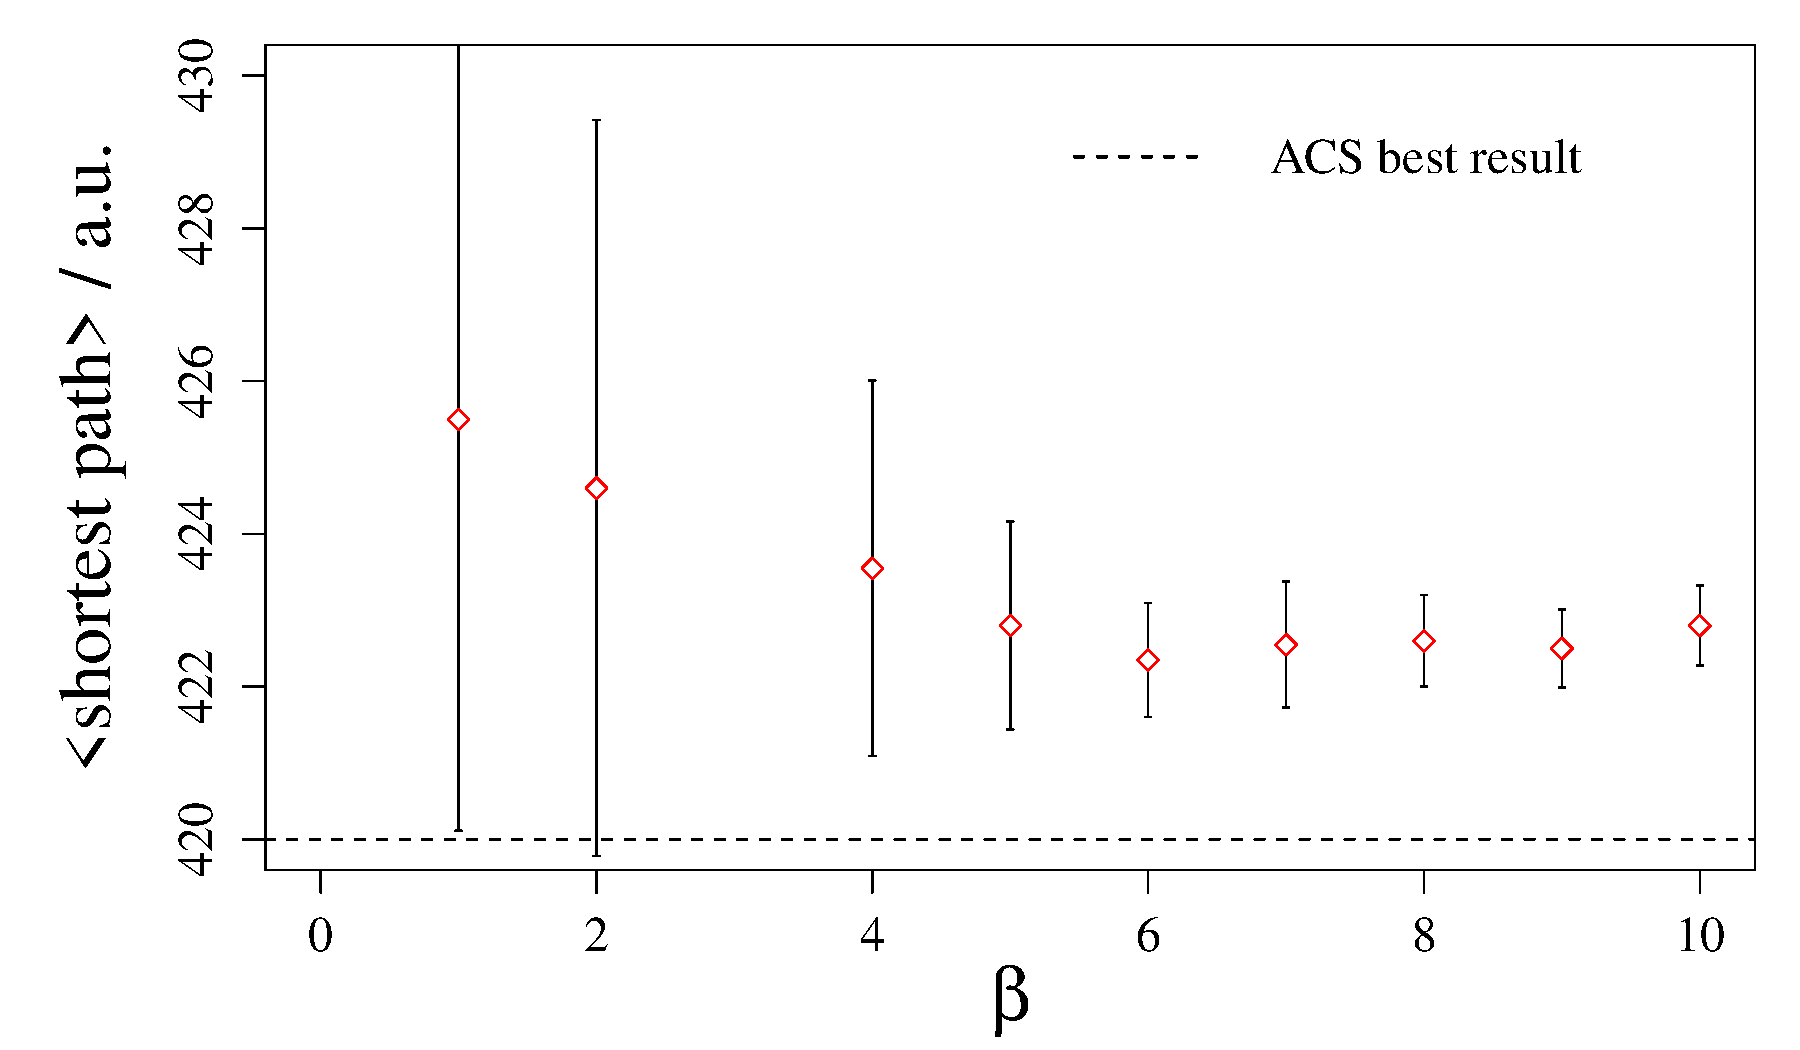
\includegraphics[width=0.8\linewidth]{beta_vs_shortestpath}
\caption{Variation of the parameter $\beta$ for the oliver30 using ten ants going 400 rounds averaged over 20 trials. The parameters are chosen as $\alpha=0.1$, $q_0=0.9$ and $\tau_{\text{start}}=0.1$.}
\label{fig:betasp}
\end{center}
\end{figure}
\noindent For the parameter $\beta$ a similar analysis has been done for a 30-city environment and ten agents. The decrease of the error for higher values of $\beta$ is explained by the fact that the criteria of closeness between the cities is weighted stronger than the pheromone concentration (see equation (\ref{eq:prob}) and (\ref{eq:qsmallerq0})). Thus, the exploration of new paths is suppressed and the deviation from the averaged path length is small. In the region of $\beta\approx2$ the bigger error bars indicate that the relative importance of pheromone and closeness is chosen such that the ants are forced to try new trails. The probability of getting stuck in a local minimum is reduced.


\subsection{Influence of the parameter $q_0$}

In Figure \ref{fig:q0zushortestpath} one can observe the influence of $q_0$ on the shortest path found after 800 rounds averaged over 10 trials for the problem \textit{oliver30}. This parameter is a measure of how random the next city is chosen (see chapter \ref{sec:model}). If the model acts with a small $q_0$ the following cities are mostly chosen randomly and do not depend strongly on the amount of pheromone on the edge or the length of the edge. As one can see a $q_0$ below 0.6 leads to a path which is a few units longer then the known solution and the error gets bigger as well. Whereas $q_0$'s in the range of 0.8 to 0.95 result in a average path which lies on the known solution and the error is vanishingly small. The problem with a $q_0 = 1$ is the fact that the ants can get stuck in a strong local minimum. The 'local' shortest path gets strongly rewarded and the edges get stronger and stronger and the ants never see a reason to change their path. Therefore one needs a certain probability that one 'crazy' ant tries some new path which can lead to a new shortest path found.\\
\newline

\begin{figure}[H]

	\centering
	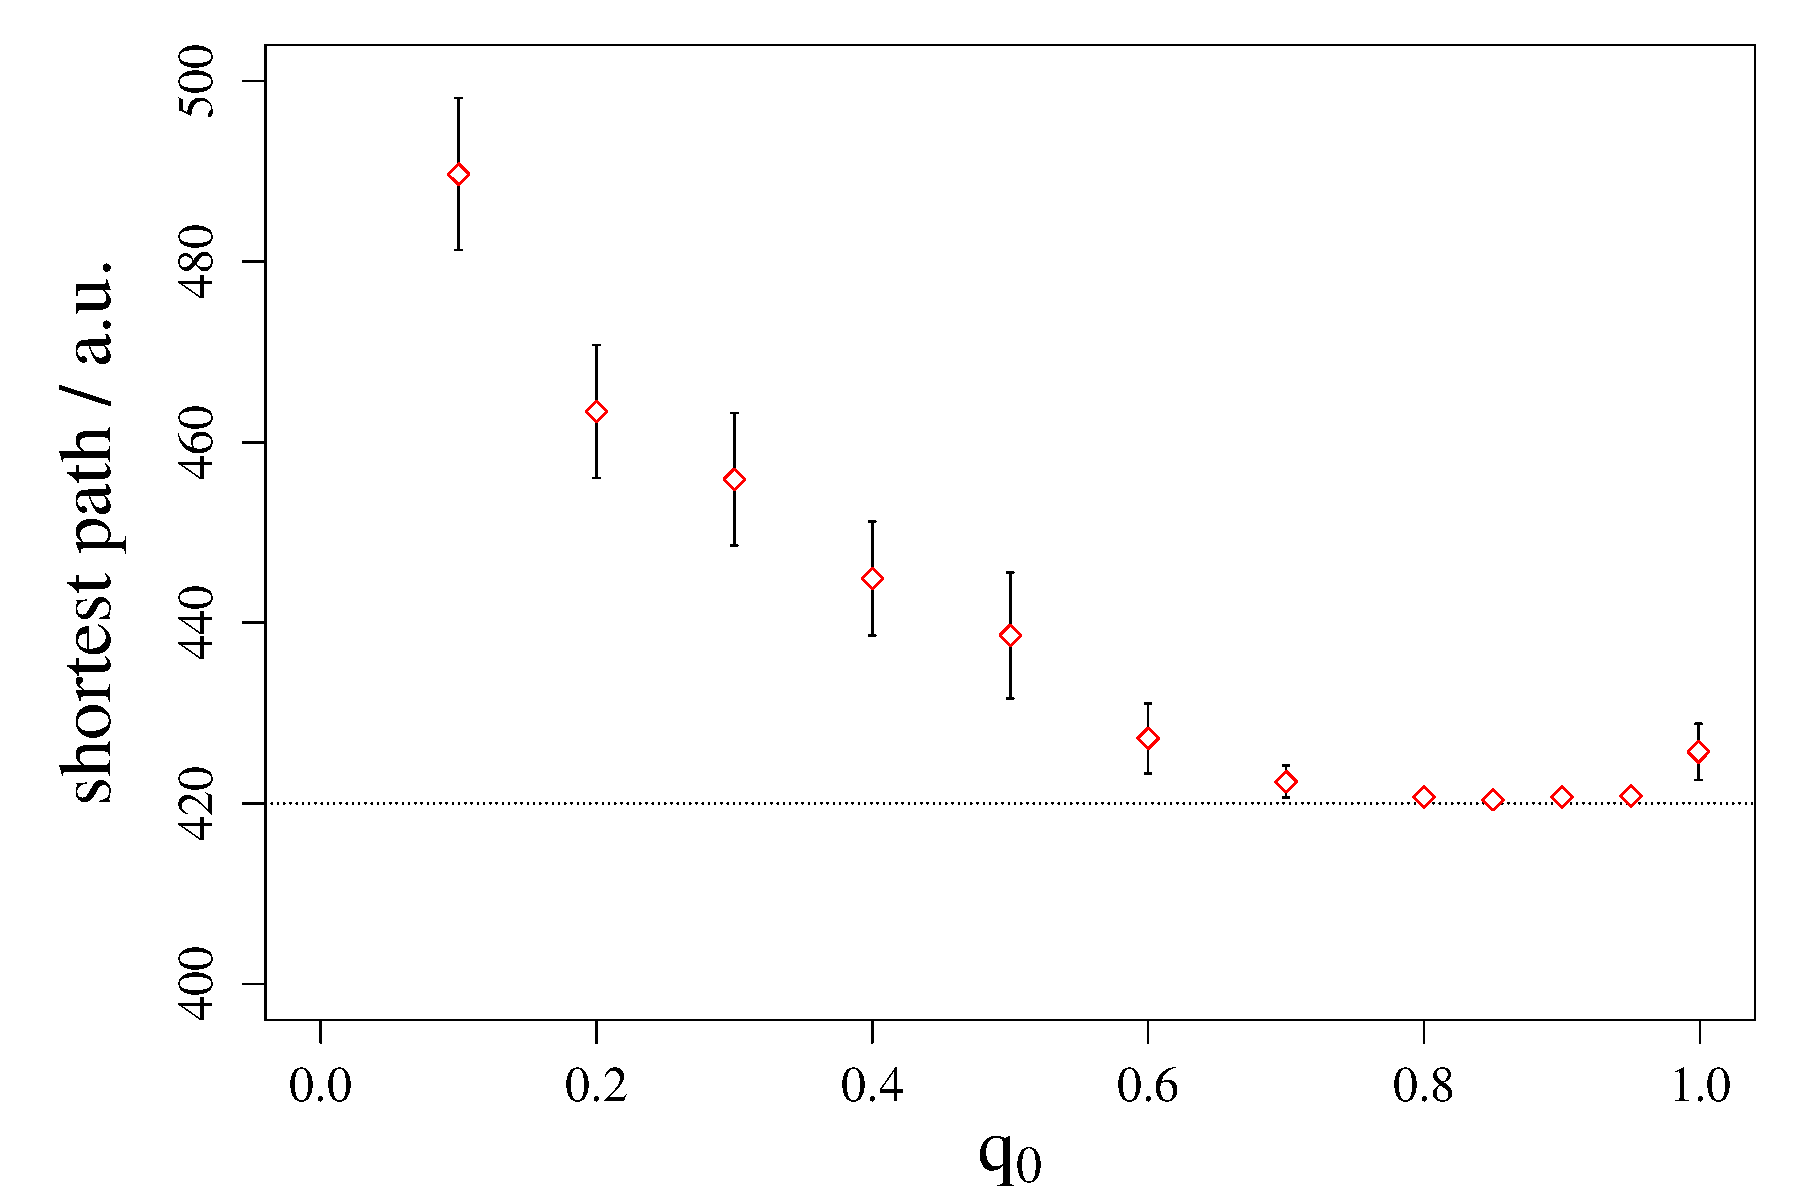
\includegraphics[width=0.8\textwidth]{Plots/q0_vs_shortestpath.pdf}

\caption{The shortest path the simulation found after 800 rounds for the problem \textit{oliver30} is plotted against the probability $q_0$ (see text for impact of $q_0$). The optimal path is shown as a dotted line along with error bars of the data. If no error bars are visible then the errors are smaller then the extent of the points.}
\label{fig:q0zushortestpath}
\end{figure}

\noindent In the appendix one can find two more graphs which investigate the behaviour of the model when changing the number of agents or the initial amount of pheromone on the edges. Both were either due to a high standard deviation useless or were not flabbergasting at all.

